\chapter{Chọn động cơ điện}
\section{Xác định công suất bộ phận công tác}
\begin{equation}
    P_{ct} = \frac{F.v}{1000} = \frac{2800 \cdot 1.4}{1000} = 3.92 \, \text{kW}
\end{equation}

\section{Số vòng quay của bộ phận công tác}
\begin{equation}
    n_{ct} = \frac{60000.v}{\pi.D} = \frac{60000 \cdot 1.4}{\pi \cdot 225} = 118.84 \, \text{(v/ph)}
\end{equation}

\section{Hiệu suất của các bộ truyền và các cặp ổ trong hệ thống dẫn động}
\begin{itemize}
    \item Bộ truyền đai: $\eta_{d} = 0.96$ 
    \item Bộ truyền bánh răng: $\eta_{br} = 0.98$
    \item Nối trục: $\eta_{nt} = 0.99$
    \item Ổ lăn: $\eta_{ol} = 0.995$
\end{itemize}
Hiệu suất hệ thống:
\begin{equation}
    \eta _{ch} = \eta_{d}\eta_{br}\eta_{nt}(\eta_{ol})^3 = 0.96 \cdot 0.98 \cdot 0.99 \cdot 0.995 = 0.9175
\end{equation}

\section{Công suất động cơ cần thiết}
\begin{equation}
    P_{dc} = \frac{P_{ct}}{\eta_{ch}} = \frac{3.92}{0.9175} = 4.273 \, \text{kW}
\end{equation}

\section{Dãy tỉ số truyền nên dùng cho các bộ truyền trong hệ thống}
\begin{itemize}
    \item Bộ truyền đai thang: $u_{d} = 2...3$
    \item Bộ truyền bánh răng trụ răng nghiêng $u_{br} = 3...5$
\end{itemize}
Như vậy số vòng quay của động cơ dao động trong khoảng từ 713 vòng/phút đến 2971 vòng/phút.\\
Chọn động cơ SGA132S có: $P_{dc} = 5.5 \, \text{kW}$ và $n_{dc} = 1450 \, \text{vòng/phút}$. \\
Như vậy tỉ số truyền chung của hệ thống là:
\begin{equation}
    u_{ch} = \frac{n_{dc}}{n_{ct}} = \frac{1450}{118.82} = 12.202
\end{equation}

\section{Phân phối tỉ số truyền}
Tỷ số truyền của cả hệ được xác định theo công thức:
\begin{equation}
    u_{ch} = u_d.u_{br} = 12.202
\end{equation}
Chọn tỉ số truyền của hộp giảm tốc:
\begin{equation}
    u_{br} = 5
\end{equation}
Như vậy:
\begin{equation}
    u_d = \frac{u_{ch}}{u_{br}} = \frac{12.202}{5} = 2.44
\end{equation}

\section{Tính toán công suất và momen trên các trục}
\subsection{Tính toán công suất trên các trục}
Công suất trên trục công tác:
\begin{equation}
    P_{ct} = \frac{F.v}{1000} = \frac{2800 \cdot 1.4}{1000} = 3.92 \, \text{kW}
\end{equation}
Công suất trên trục II:
\begin{equation}
    P_{II} = \frac{P_{ct}}{\eta_{ol}^2.\eta_{nt}} = \frac{3.92}{0.995^2 \cdot 0.99} = 4 \, \text{kW}
\end{equation}
Công suất trên trục I:
\begin{equation}
    P_{I} = \frac{P_{II}}{\eta_{ol} \cdot \eta_{br}} = \frac{4}{0.995 \cdot 0.98} = 4.102 \, \text{kW}
\end{equation}

\subsection{Tính toán momen trên các trục}
Momen trên trục công tác:
\begin{equation}
    M_{lv} = 9.55 \cdot 10^6 \cdot \frac{P_{ct}}{n_{ct}} = 9.55 \cdot 10^6 \cdot \frac{3.92}{118.82} = 315053.5 \, \text{(N.mm)}
\end{equation}
Momen trên trục II:
\begin{equation}
    M_{II} = 9.55 \cdot 10^6 \cdot \frac{P_{II}}{n_{II}} = 9.55 \cdot 10^6 \cdot \frac{4}{118.82} = 321442.24 \, \text{(N.mm)}
\end{equation}
Momen trên trục I:
\begin{equation}
    M_{I} = 9.55 \cdot 10^6 \cdot \frac{P_{I}}{n_{I}} = 9.55 \cdot 10^6 \cdot \frac{4.102}{594.26} = 65914.97 \, \text{(N.mm)}
\end{equation}
Momen trên trục động cơ:
\begin{equation}
    M_{dc} = 9.55 \cdot 10^6 \cdot \frac{P_{dc}}{n_{dc}} = 9.55 \cdot 10^6 \cdot \frac{4.275}{1450} = 28139.71 \, \text{(N.mm)}
\end{equation}

\section{Bảng thông số hệ thống}
\begin{figure}[H]
    \centering
    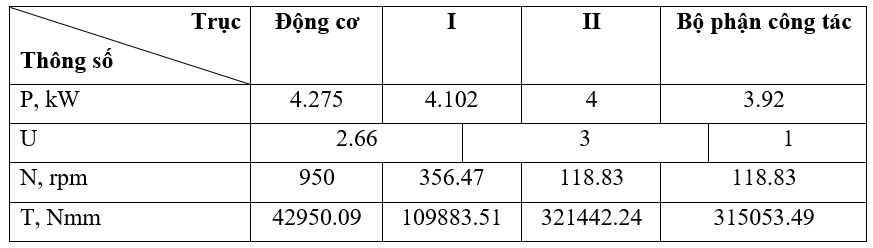
\includegraphics[width=1\textwidth]{pictures/bangdactinh.png}
    \caption{Bảng thông số hệ thống}
\end{figure}